\begin{apendicesenv} % Imprime uma página indicando o início dos apêndices

  \chapter*{Formulário de pesquisa}

  \section{Formulário de pesquisa} % ### 4.4. % Adicionar as imagens do formulário

  % CORRIGIR FUTURAMENTE - XXX Checar se as perguntas nas tabelas, prints e anexo são as mesmas

  Como forma de analisar também a perspectiva dos discentes quanto à problemática abordada, foi elaborado um formulário de pesquisa com o intuito de se confirmar ou não a hipótese de que em sua maioria os alunos também se encontram insatisfeitos com a atual conjuntura de distribuição e alocação de turmas.

  Para este fim, foi utilizado um formulário de pesquisa qualitativa dos alunos disponível no Apêndice 1. O formulário foi divulgado através de um link disponibilizado no grupo de alunos do curso de Ciência da Computação no WhatsApp, e também através de um link distribuído pela Secretaria Acadêmica a discentes da UENF.

  A seguir, estão dispostos alguns resultados obtidos pelo formulário.

  \section*{Respondentes} \label{sec:Respondentes}

  Inicialmente foram solicitadas algumas informações dos alunos, como seu curso, ano de ingresso. As respostas estão dispostas na \autoref{table:2.1_SobreVoce_Cursos}.

  % \begin{MyCenteredFigure} \caption{Perguntas sobre o curso e ano de ingresso dos estudantes} \label{fig:2.0-SobreVoce}
  %   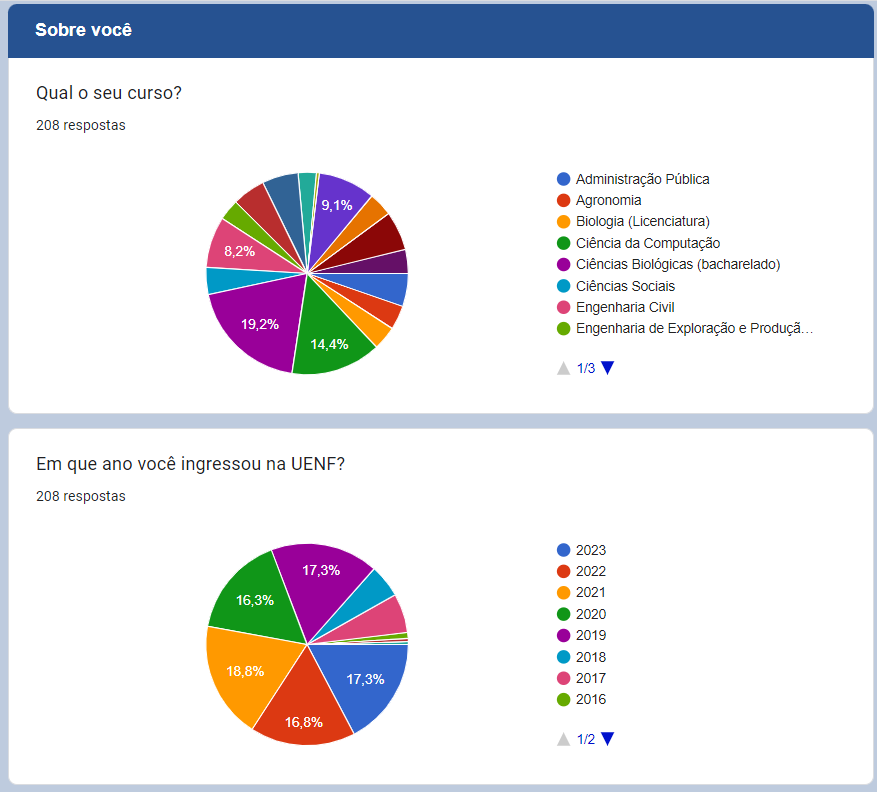
\includegraphics[width=\textwidth]{files/img/2.02!3-organizacao/2.02!3.1.4-forms/2.0-SobreVoce}
  % \end{MyCenteredFigure}

  O formulário foi respondido por 208 alunos, sendo os cursos de maior incidência o bacharelado de Ciências Biológicas com 40 respondentes, Ciência da Computação com 29 e Medicina Veterinária com 19. Vale ressaltar que 96 dos respondentes são alunos de cursos que envolvem diretamente o CCT. Entretanto, a análise dos gráficos abordará a percepção de todos igualmente.

  \begin{CenteredTable} \caption{Número de respondentes por curso} \label{table:2.1_SobreVoce_Cursos}
    \begin{tabular}{| r r l |}
      \hline
      \textbf{Quantidade} & \%   & \textbf{Curso}                                  \\
      \hline
      40                  & 19,3 & Ciências Biológicas (bacharelado)               \\
      29                  & 14,0 & Ciência da Computação                           \\
      19                  & 9,2  & Medicina Veterinária                            \\
      17                  & 8,2  & Engenharia Civil                                \\
      13                  & 6,3  & Química (Licenciatura)                          \\
      12                  & 5,8  & Engenharia Metalúrgica                          \\
      11                  & 5,3  & Engenharia de Produção                          \\
      11                  & 5,3  & Administração Pública                           \\
      9                   & 4,3  & Ciências Sociais                                \\
      8                   & 3,9  & Agronomia                                       \\
      8                   & 3,9  & Biologia (Licenciatura)                         \\
      8                   & 3,9  & Pedagogia (Licenciatura)                        \\
      8                   & 3,9  & Zootecnia                                       \\
      7                   & 3,4  & Engenharia de Exploração e Produção de Petróleo \\
      6                   & 2,9  & Física (licenciatura)                           \\
      1                   & 0,5  & Matemática (Licenciatura)                       \\
      0                   & 0,0  & Engenharia Meteorológica                        \\
      0                   & 0,0  & Outro                                           \\
      \hline
    \end{tabular}
  \end{CenteredTable}

  Vemos também a distribuição dos anos de ingresso dos alunos que responderam o formulário, sendo seu quantitativo bem distribuído entre os anos de 2019 e 2023, tendo os anos de 2017 e 2018 uma quantidade menor de respostas, os outros anos tendo em conjunto um total de 4 respostas (\autoref{table:2.2_SobreVoce_Anos}).

  \begin{CenteredTable} \caption{Número de respondentes por ano} \label{table:2.2_SobreVoce_Anos}
    \begin{tabular}{| c r c |}
      \hline
      \textbf{Quantidade} & \%   & \textbf{Ano} \\
      \hline
      36                  & 17,4 & 2023         \\
      35                  & 16,9 & 2022         \\
      39                  & 18,8 & 2021         \\
      34                  & 16,4 & 2020         \\
      35                  & 16,9 & 2019         \\
      11                  & 5,3  & 2018         \\
      13                  & 6,3  & 2017         \\
      2                   & 1,0  & 2016         \\
      1                   & 0,5  & 2015         \\
      0                   & 0,0  & 2014         \\
      0                   & 0,0  & 2013         \\
      1                   & 0,5  & Outro        \\
      \hline
    \end{tabular}
  \end{CenteredTable}

  \section*{Avaliação de experiência acadêmica} \label{sec:Avaliação de experiência acadêmica}

  Considerando que o escopo deste trabalho revolve em torno da alocação de recursos físicos e humanos, como salas, professores e alunos, foi elaborada uma seção do formulário de pesquisa com o intuito de se analisar a frequência de ocorrência de certas situações no contexto universitário. Para isto, foram feitas as seguintes perguntas:

  \begin{enumerate}
    \item Salas: Você já teve que mudar de sala por falta de algum acessório como quadro, projetor ou monitor? % 53.1%
    \item Salas: Você já teve aula cuja sala não dispunha de carteiras o suficiente? % 52.7%
    \item Vagas: Você já quis entrar em uma disciplina, mas ela não tinha vaga? % 85.0%
    \item Vagas: Você já ficou acordado após meia-noite por medo de não ter vaga para as disciplinas que deseja cursar? % 91.3%
    \item Conflitos: Você já deixou de se inscrever em uma disciplina por causa de conflito de horário? % 90.8%
    \item Preferências: Você já preferiu não se inscrever em uma disciplina para cursá-la em outro momento mais oportuno? % 86.0%
    \item Opiniões: Você acha que a universidade deveria oferecer horários diferentes para as disciplinas mais demandadas para evitar conflitos com outras  % 100.0%
  \end{enumerate}

  A enumeração das perguntas feitas se encontra representada com suas respectivas respostas na \autoref{table:3.0_satisfacao}.

  \begin{CenteredTable} \caption{Ocorrência de experiências acadêmicas} \label{table:3.0_satisfacao}
    \begin{tabular}{| c | c c c | r r r |}
      \hline
      \multicolumn{1}{|c|}{\multirow{2}{*}{Pergunta}} & \multicolumn{3}{c|}{Respostas} & \multicolumn{3}{c|}{Respostas (\%)}                                                                  \\
      \multicolumn{1}{|c|}{}                          & Sim                            & \multicolumn{1}{|c|}{Não}           & Outro & Sim (\%) & \multicolumn{1}{|c|}{Não (\%)} & Outro (\%) \\
      \hline
      1                                               & 110                            & 87                                  & 10    & 53,1     & 42,0                           & 4,8        \\ % 110/207=0.5314 =  53.1%
      2                                               & 109                            & 95                                  & 3     & 52,7     & 45,9                           & 1,4        \\ % 109/207=0.5265 =  52.7%
      3                                               & 176                            & 28                                  & 3     & 85,0     & 13,5                           & 1,4        \\ % 176/207=0.8502 =  85.0%
      4                                               & 189                            & 17                                  & 1     & 91,3     & 8,2                            & 0,5        \\ % 189/207=0.9130 =  91.3%
      5                                               & 188                            & 15                                  & 4     & 90,8     & 7,2                            & 1,9        \\ % 188/207=0.9082 =  90.8%
      6                                               & 178                            & 27                                  & 2     & 86,0     & 13,0                           & 1,0        \\ % 178/207=0.8599 =  86.0%
      7                                               & 207                            & 0                                   & 0     & 100,0    & 0,0                            & 0,0        \\ % 207/207=1.0000 = 100.0%
      \hline
    \end{tabular}
  \end{CenteredTable}

  % \begin{MyCenteredFigure} \caption{Respostas sobre a satisfação dos estudantes} \label{fig:3.0_Satisfacao}
  %   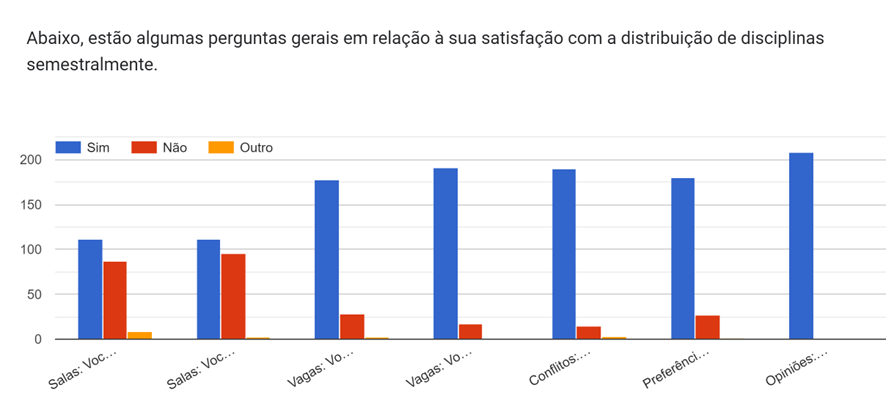
\includegraphics[width=\textwidth]{files/img/2.02!3-organizacao/2.02!3.1.4-forms/3.0-Satisfacao}
  % \end{MyCenteredFigure}

  Quanto à distribuição dos recursos físicos, vemos uma taxa de 53,1\% de alunos que já tiveram que mudar de sala por falta de algum acessório disposto necessário para a aula. Já a necessidade de mudança de sala devido à ausência de carteiras suficientes obteve taxa de 52,7\%.

  É notório o receio dos alunos quanto à possibilidade de não conseguir se inscrever nas disciplinas que desejam cursar, tendo sido confirmado por 85,0\% dos respondentes que se viram em situação em que a disciplina na qual desejavam se matricular não dispunha de vagas o bastante. Essa realidade resulta no temor por semestralmente não conseguir se inscrever na disciplina desejada, fazendo com que 91,3\% dos respondentes tenham se mantido acordados após a meia-noite por causa deste medo.

  O temor de não conseguir se inscrever nas disciplinas desejadas é ainda agravado pelo fato de que 90,8\% dos alunos que já deixaram de se inscrever em disciplinas devido a conflitos de horário.

  O que se apresenta como um agravante ainda maior na percepção da progressão não sequencial dos alunos é a quantidade de alunos que já preferiram não se inscrever em uma disciplina para cursá-la em outro momento mais oportuno, mesmo que isto signifique um atraso na progressão do curso, sendo seu percentual 86,0\%.

  Embora seja uma prática recorrente a oferta de diversas turmas para uma mesma disciplina, o que usualmente é feito de forma que as turmas sejam ofertadas no mesmo horário. Entretanto, os alunos, unanimemente, não se mostram satisfeitos com esta prática, visto que 100\% dos respondentes consideram que a universidade deveria dispor de outros horários para as disciplinas mais demandadas com o intuito de evitar conflitos de horários.

  Este resultado é curioso, visto que o temor de não se atrasar em seu progresso e conseguir se inscrever nas disciplinas desejadas, contrasta diretamente com a preferência pessoal de não se inscrever em disciplinas e cursá-las posteriormente, mesmo que isso possa atrasar seu progresso. Entende-se que nem todas as disciplinas, caso não cursadas em seu período esperado, resultarão no atraso da grade, mas ainda assim, a antítese é evidente.

  \section*{Preferências pessoais} \label{sec:Preferências pessoais}

  Neste segmento, visa-se entender um pouco melhor o processo decisório dos alunos quanto à escolha das disciplinas que desejam cursar. Primeiro, lhes é indagado quanto à disposição das disciplinas, variando entre disciplinas concentradas em poucos dias ou espalhadas durante a semana e quanto à preferência de horários, variando entre horários matutinos e vespertinos.

  Embora não lide com conflitos, a análise de seus resultados pode auxiliar na escolha de distribuição futura dos usuários do sistema, ao desenvolverem a grade horária, caso desejem considerar as preferências dos estudantes.

  \begin{comment}
  \begin{MyCenteredFigure} \caption{Preferências por distribuição de disciplinas ao longo da semana} \label{fig:4.1-PreferenciasPessoais-Distribuida_Acumulada}
    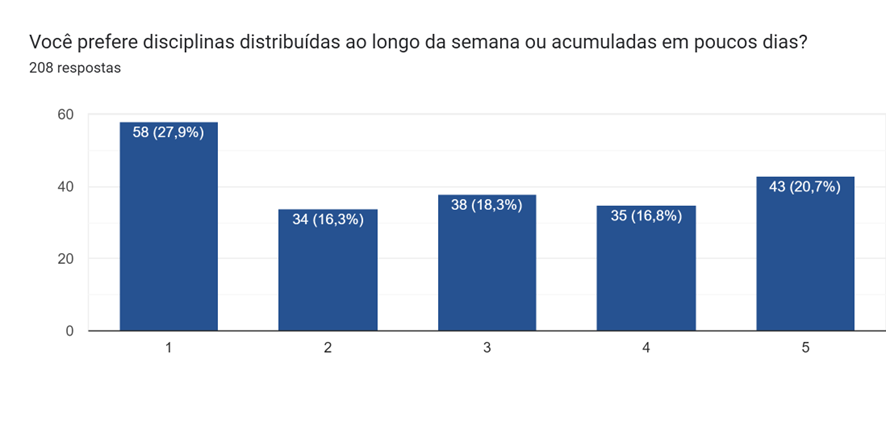
\includegraphics[width=\textwidth]{files/img/2.02!3-organizacao/2.02!3.1.4-forms/4.1-PreferenciasPessoais-Distribuida_Acumulada}
  \end{MyCenteredFigure}

  \begin{MyCenteredFigure} \caption{Preferências por distribuição de disciplinas em um mesmo dia} \label{fig:4.2-PreferenciasPessoais-Manha_Tarde}
    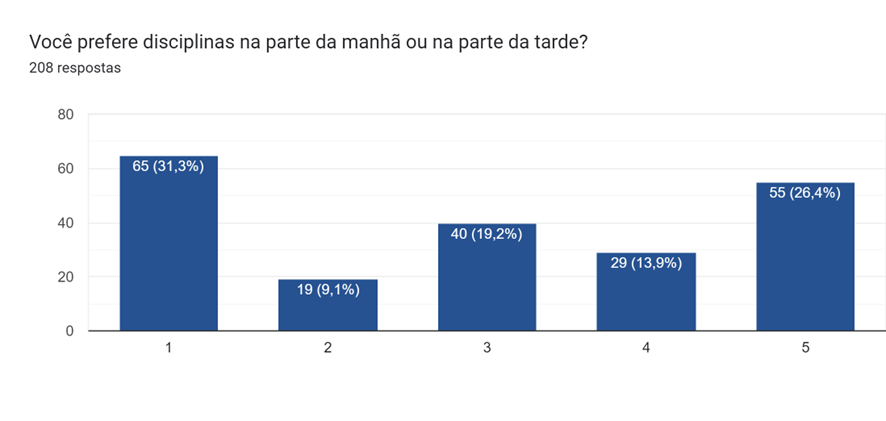
\includegraphics[width=\textwidth]{files/img/2.02!3-organizacao/2.02!3.1.4-forms/4.2-PreferenciasPessoais-Manha_Tarde}
  \end{MyCenteredFigure}
  \end{comment}

  Podemos ver na \autoref{table:4.1-PreferenciasPessoais-Distribuída_Acumulada} que há uma grande distribuição entre as preferências dos alunos, tendendo às extremidades, onde alguns preferem bastante as disciplinas distribuídas ao longo da semana enquanto outros preferem disciplinas acumuladas em poucos dias, vindo como terceira opção mais votada a neutralidade. Observação similar se mostra presente também na \autoref{table:4.2-PreferenciasPessoais-Manha_Tarde}.

  Como alternativa de visualização, dispomos aqui da \autoref{table:4.1-PreferenciasPessoais-Distribuída_Acumulada} e da \autoref{table:4.2-PreferenciasPessoais-Manha_Tarde} com os resultados numéricos.

  \begin{CenteredTable} \caption{Preferências por distribuição de disciplinas em um mesmo dia} \label{table:4.1-PreferenciasPessoais-Distribuída_Acumulada}
    \begin{tabular}{| r r l |}
      \hline
      \textbf{Quantidade} & \%   & \textbf{Distribuição na semana}            \\
      \hline
      58                  & 28,0 & Distribuídas ao longo da semana            \\
      34                  & 16,4 & Preferencialmente ao longo da semana       \\
      38                  & 18,4 & Não tenho preferência                      \\
      35                  & 16,9 & Preferencialmente acumulada em poucos dias \\
      42                  & 20,3 & Acumuladas em poucos dias                  \\
      \hline
    \end{tabular}
  \end{CenteredTable}

  \begin{CenteredTable} \caption{Preferências por distribuição de disciplinas em um mesmo dia} \label{table:4.2-PreferenciasPessoais-Manha_Tarde}
    \begin{tabular}{| r r l |}
      \hline
      \textbf{Quantidade} & \%   & \textbf{Distribuição no dia}        \\
      \hline
      65                  & 31,4 & Na parte da manhã                   \\
      19                  & 9,2  & Preferencialmente na parte da manhã \\
      40                  & 19,3 & Não tenho preferência               \\
      28                  & 13,5 & Preferencialmente na parte da tarde \\
      55                  & 26,6 & Na parte da tarde                   \\
      \hline
    \end{tabular}
  \end{CenteredTable}

  Em seguida, é questionado sobre qual é o critério de seleção de disciplinas que se apresentam conflituosas (\autoref{table:4.3-PreferenciasPessoais-Conflitos}). Nesta vertente vemos uma maior propensão às disciplinas que é pré-requisito de uma grande quantidade de disciplinas, ou seja, disciplinas que, caso se tenham reprovação ou não sejam cursadas, resultam no que é coloquialmente chamado de ``prender disciplinas'', assim atrasando mais a progressão do aluno. Sendo este o critério adotado por 81,3\% dos respondentes. A segunda maior opção selecionada foi a de escolher a disciplina mais concorrida, ou seja, a disciplina que possui uma maior demanda de alunos, sendo um critério utilizado por 25\% dos alunos. Os valores exatos podem ser vistos na \autoref{table:4.3-PreferenciasPessoais-Conflitos}.

  % \begin{MyCenteredFigure} \caption{Critérios para a escolha de disciplinas conflituosas} \label{fig:4.3-PreferenciasPessoais-Conflitos}
  %   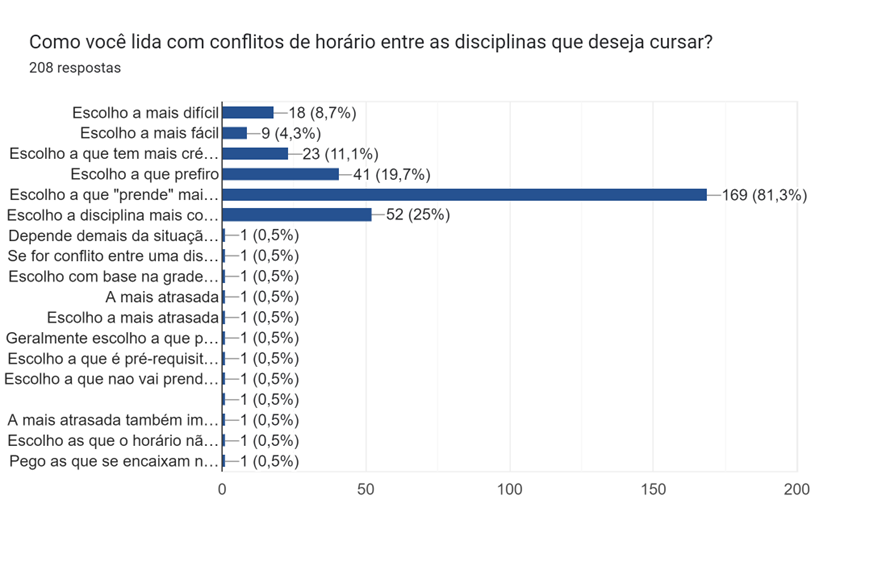
\includegraphics[width=\textwidth]{files/img/2.02!3-organizacao/2.02!3.1.4-forms/4.3-PreferenciasPessoais-Conflitos}
  % \end{MyCenteredFigure}

  Vale ressaltar que as respostas ilustradas pela \autoref{fig:4.3-PreferenciasPessoais-Conflitos} permite a seleção de múltiplas escolhas, inclusive permitindo que adicionassem outros critérios próprios. Dentre eles, um se mostrou ligeiramente recorrente que seria escolher a disciplina mais atrasada segundo a grade curricular. Outra possibilidade citada foi selecionar a que se encaixam na disponibilidade de horário pessoal, para que não conflite, por exemplo, com o horário do estágio obrigatório.

  \begin{CenteredTable} \caption{Critérios para a escolha de disciplinas conflituosas} \label{table:4.3-PreferenciasPessoais-Conflitos}
    \begin{tabular}{| r r l |}
      \hline
      \textbf{Quantidade} & \%   & \textbf{Forma de escolher disciplina conflituosa} \\
      \hline
      169                 & 81,6 & Escolho a que ``prende'' mais matérias            \\
      52                  & 25,1 & Escolho a disciplina mais concorrida              \\
      41                  & 19,8 & Escolho a que prefiro                             \\
      23                  & 11,1 & Escolho a que tem mais créditos                   \\
      18                  & 8,7  & Escolho a mais difícil                            \\
      12                  & 5,8  & Outro                                             \\
      9                   & 4,3  & Escolho a mais fácil                              \\
      \hline
    \end{tabular}
  \end{CenteredTable}

  \section*{Experiências com atrasos e disciplinas} \label{sec:Experiências com atrasos e disciplinas}

  Quanto aos atrasos para a realização de disciplinas, o ideal desejado é que não haja nenhum atraso. Nessa situação, todos os alunos que entram na universidade poderão seguir a disponibilidade usual das disciplinas dispostas em suas grades curriculares, que apresentam o período esperado para que cada disciplina seja realizada. Sendo elas, usualmente dividas como disciplinas pares e ímpares. As ímpares se referem às disciplinas em que se espera que sejam cursadas nos períodos 1, 3, 5, 7 e 9, e que são ofertadas no primeiro semestre letivo. Enquanto que as pares se referem às disciplinas oferecidas no segundo período letivo, onde geralmente se alocam as disciplinas dos períodos 2, 4, 6, 8 e 10.

  Entretanto, a realidade dos alunos é outra. Isso se dá por diversos motivos, seja por reprovação, por não conseguir se inscrever na disciplina desejada ou por simplesmente não ter interesse em cursar a disciplina naquele momento, como já ilustrado na \autoref{table:3.0_satisfacao}. Esta característica se confirma na percepção da frequência e distância que percebemos dos atrasos, representado pela \autoref{table:5.0-Atrasos}.

  \begin{comment}
  \begin{MyCenteredFigure} \caption{Períodos de atraso por espera} \label{fig:5.1-Atrasos-Esperar}
    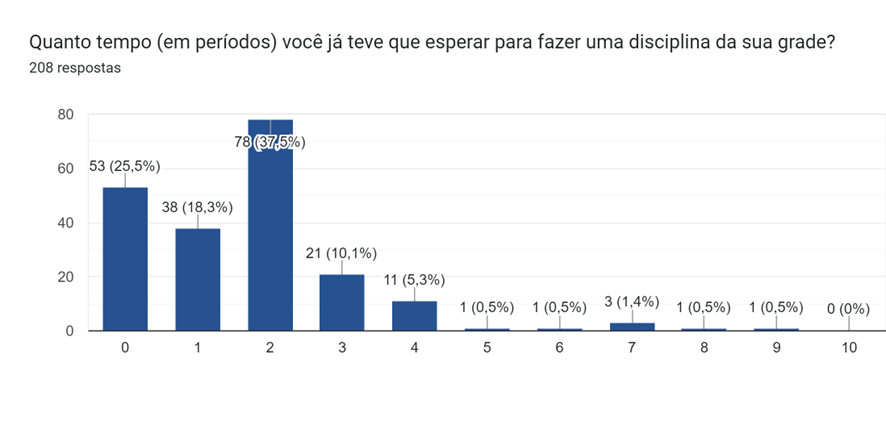
\includegraphics[width=\textwidth]{files/img/2.02!3-organizacao/2.02!3.1.4-forms/5.1-Atrasos-Esperar}
  \end{MyCenteredFigure}

  \begin{MyCenteredFigure} \caption{Distância de atraso} \label{fig:5.2-Atrasos-Distancia}
    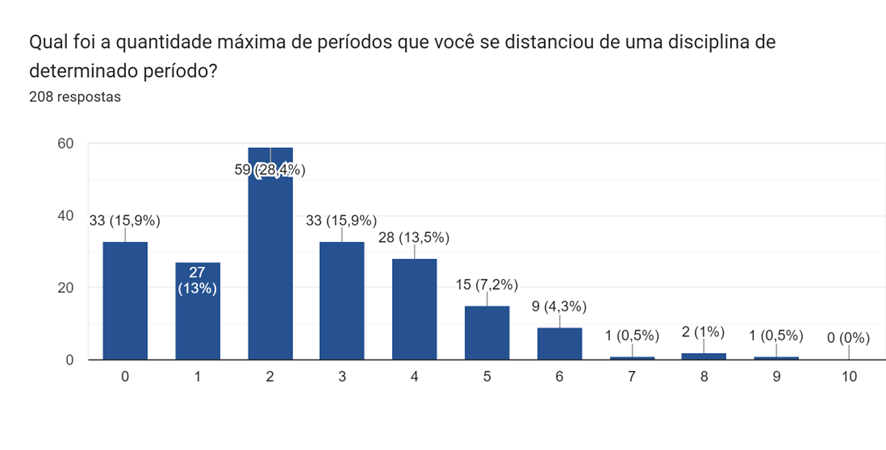
\includegraphics[width=\textwidth]{files/img/2.02!3-organizacao/2.02!3.1.4-forms/5.2-Atrasos-Distancia}
  \end{MyCenteredFigure}
  \end{comment}

  Apresenta-se notável que é minoria a quantidade de alunos que nunca tiveram que esperar para cursar uma disciplina, sendo estes apenas 25,5\% dos respondentes. É ainda mais notável o fato de que o tempo de espera médio é de mais de um ano e meio. Quanto ao distanciamento de disciplinas, seja por reprovações ou por escolha própria se mostra ainda mais presente, sendo que apenas 15,9\% dos respondentes não se distanciaram das disciplinas esperadas para o período, sendo 2.8 anos o tempo médio de distanciamento.

  Abaixo, encontra-se disposto na \autoref{table:5.0-Atrasos} os resultados obtidos através desta seção do formulário.

  \begin{enumerate}
    \item Quanto tempo (em períodos) você já teve que esperar para fazer uma disciplina da sua grade?
    \item Qual foi a quantidade máxima de períodos que você se distanciou de uma disciplina de determinado período?
  \end{enumerate}

  \begin{CenteredTable} \caption{Tempo de atraso em disciplinas} \label{table:5.0-Atrasos}
    \begin{tabular}{| c | c c c c c c c c c c c |}
      \hline
      \multicolumn{1}{|c|}{\multirow{2}{*}{Pergunta}} &
      \multicolumn{11}{c|}{Períodos de atraso}                                                          \\
      \multicolumn{1}{|c|}{}                          &
      \multicolumn{1}{c|}{0}                          &
      \multicolumn{1}{c|}{1}                          &
      \multicolumn{1}{c|}{2}                          &
      \multicolumn{1}{c|}{3}                          &
      \multicolumn{1}{c|}{4}                          &
      \multicolumn{1}{c|}{5}                          &
      \multicolumn{1}{c|}{6}                          &
      \multicolumn{1}{c|}{7}                          &
      \multicolumn{1}{c|}{8}                          &
      \multicolumn{1}{c|}{9}                          &
      \multicolumn{1}{|c|}{10}
      \\
      \hline
      1                                               & 53   & 38   & 79   & 19   & 11   & 1   & 1   & 3   & 1   & 1   & 0   \\
      2                                               & 33   & 27   & 60   & 31   & 28   & 15  & 9   & 1   & 2   & 1   & 0   \\
      \hline
      1 (\%)                                          & 25,6 & 18,4 & 38,2 & 9,2  & 5,3  & 0,5 & 0,5 & 1,4 & 0,5 & 0,5 & 0,0 \\
      2 (\%)                                          & 15,9 & 13,0 & 29,0 & 15,0 & 13,5 & 7,2 & 4,3 & 0,5 & 1,0 & 0,5 & 0,0 \\
      \hline
    \end{tabular}
  \end{CenteredTable}

  \section*{Pesquisa de opinião} \label{sec:Pesquisa de opinião}

  Aqui, buscamos uma análise mais bruta e direta à concordância dos respondentes quanto às características atribuídas à distribuição de disciplinas semestrais, ondem eles avaliam com notas de 1 a 5 o quanto concordam com cada uma das características dadas à distribuição de disciplinas, sendo eles ``Justa'', ``Variada'', ``Contínua'', ``Eficiente'', ``Distribuída'' e ``Satisfatória''. Estando as opiniões dos alunos refletidas nos resultados expostos pela \autoref{table:6.0-Opiniao}.

  \begin{comment}
  \begin{MyCenteredFigure} \caption{Notas dadas para as características da distribuição de disciplinas} \label{fig:6.0-Opiniao-Todas}
    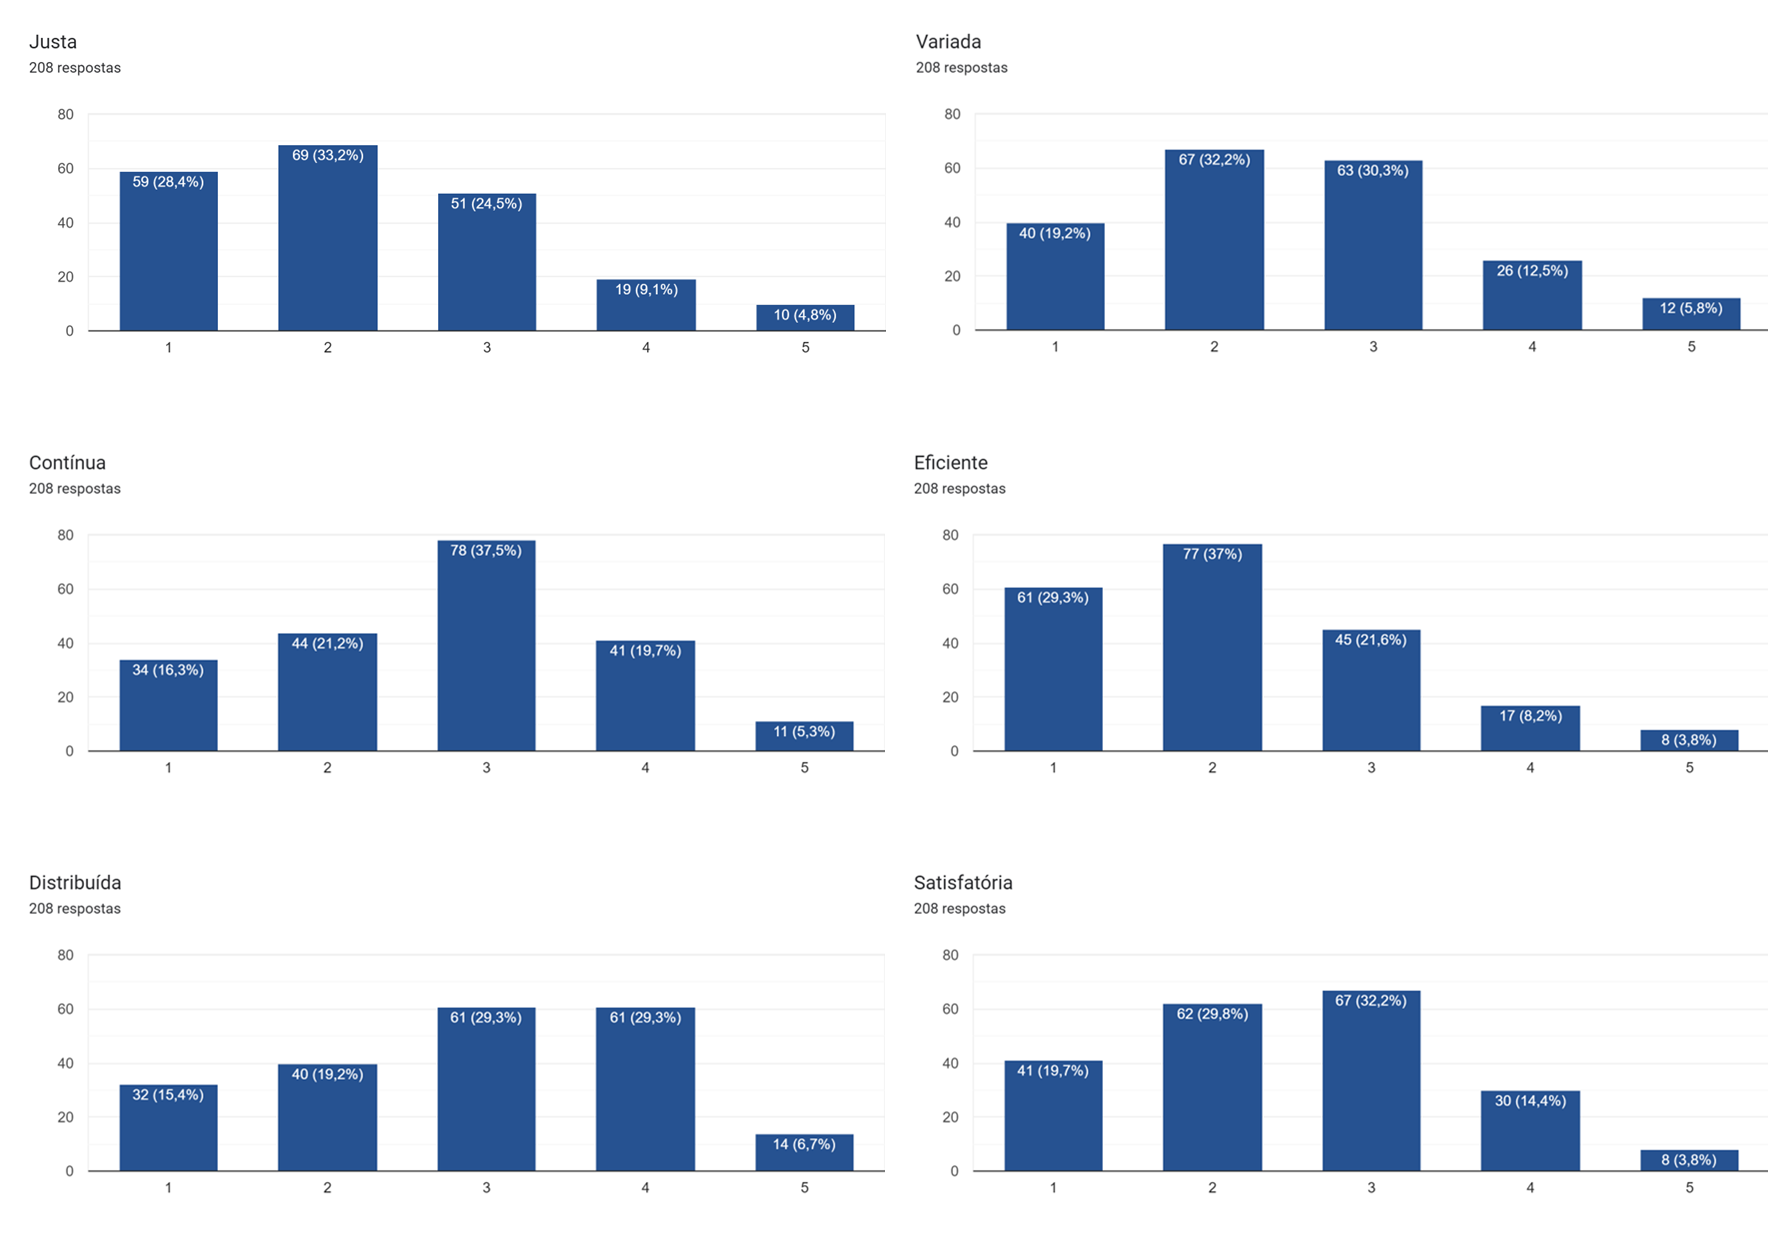
\includegraphics[width=\textwidth]{files/img/2.02!3-organizacao/2.02!3.1.4-forms/6.0-Opiniao-Todas}
  \end{MyCenteredFigure}

  \begin{MyCenteredFigure} \caption{Resultados das características ``Justa'', ``Variada'' e ``Contínua''} \label{fig:6.0-Opiniao-1_3}
    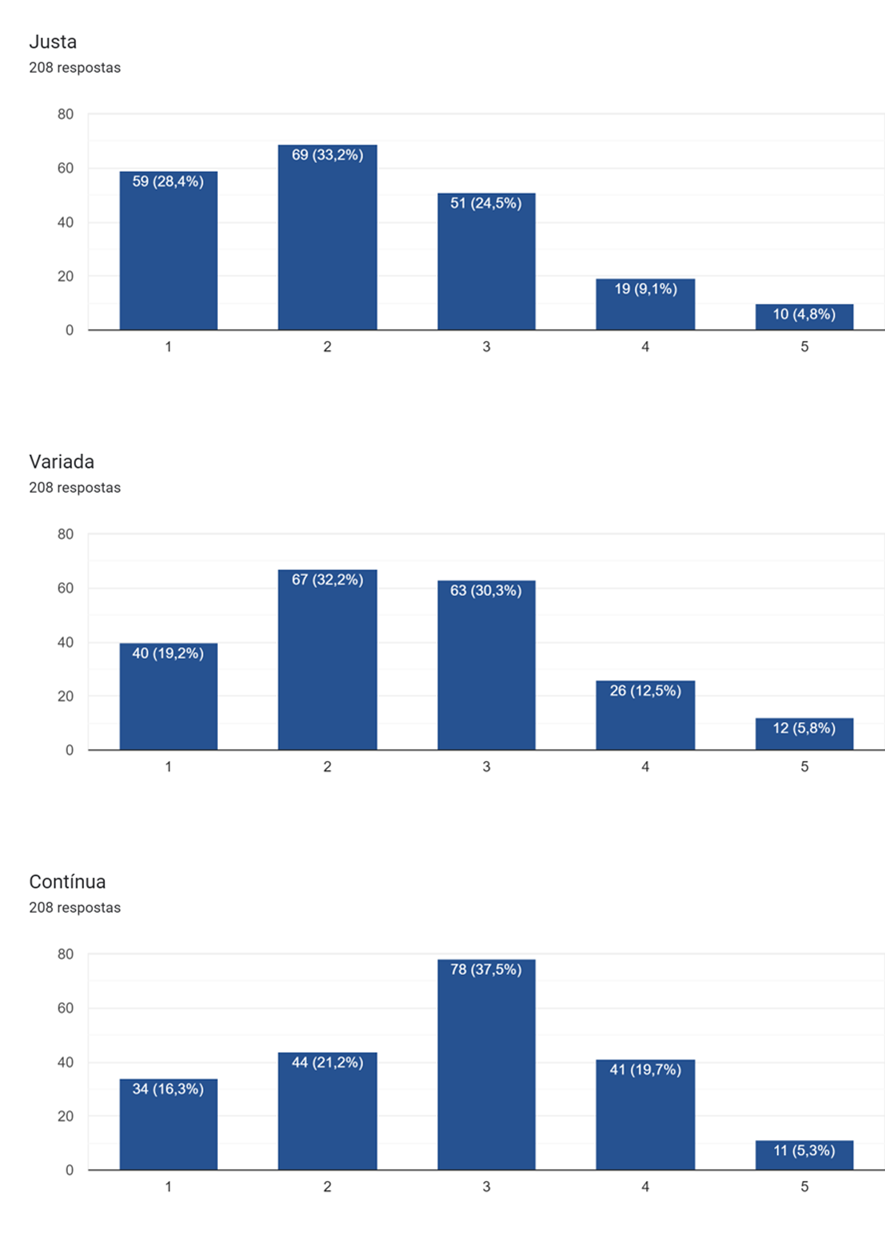
\includegraphics[width=\textwidth]{files/img/2.02!3-organizacao/2.02!3.1.4-forms/6.0-Opiniao-1_3}
  \end{MyCenteredFigure}

  \begin{MyCenteredFigure} \caption{Resultados das características ``Eficiente'', ``Distribuída'' e ``Satisfatória''} \label{fig:6.0-Opiniao-4_6}
    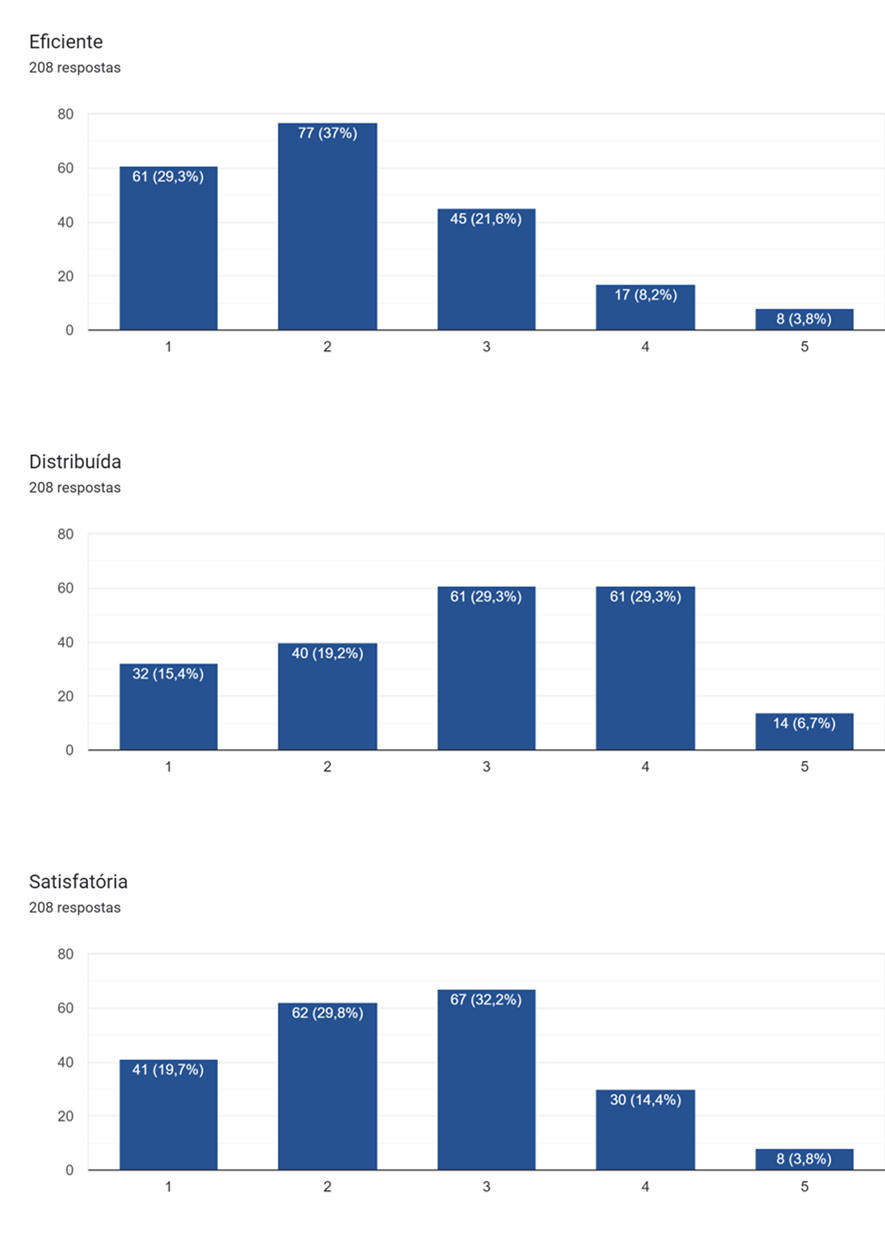
\includegraphics[width=\textwidth]{files/img/2.02!3-organizacao/2.02!3.1.4-forms/6.0-Opiniao-4_6}
  \end{MyCenteredFigure}

  \begin{MyCenteredFigure} \caption{Notas dadas para a característica: justa} \label{fig:6.1-Opiniao-Justa}
    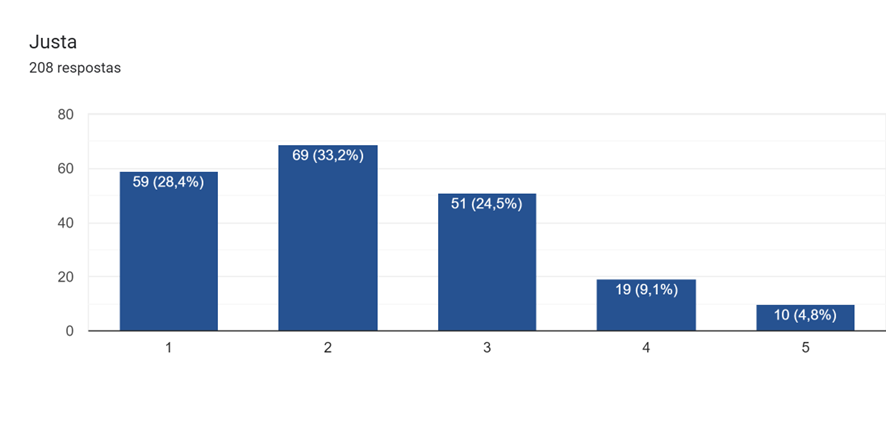
\includegraphics[width=\textwidth]{files/img/2.02!3-organizacao/2.02!3.1.4-forms/6.1-Opiniao-Justa}
  \end{MyCenteredFigure}

  \begin{MyCenteredFigure} \caption{Notas dadas para a característica: variada} \label{fig:6.2-Opiniao-Variada}
    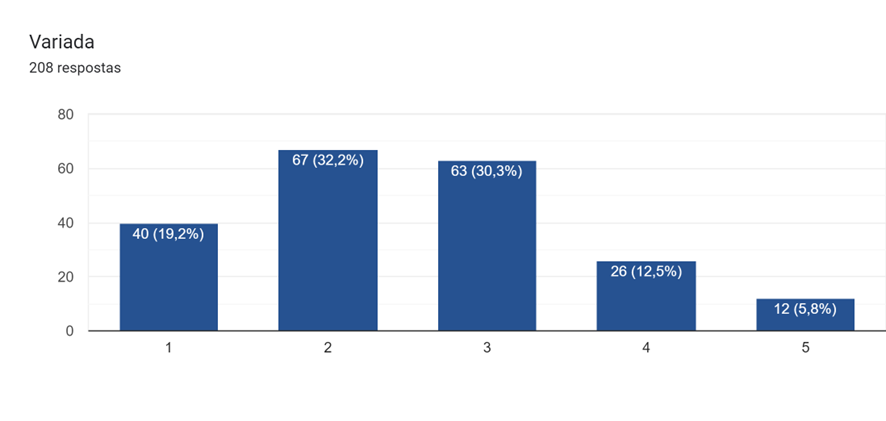
\includegraphics[width=\textwidth]{files/img/2.02!3-organizacao/2.02!3.1.4-forms/6.2-Opiniao-Variada}
  \end{MyCenteredFigure}

  \begin{MyCenteredFigure} \caption{Notas dadas para a característica: contínua} \label{fig:6.3-Opiniao-Continua}
    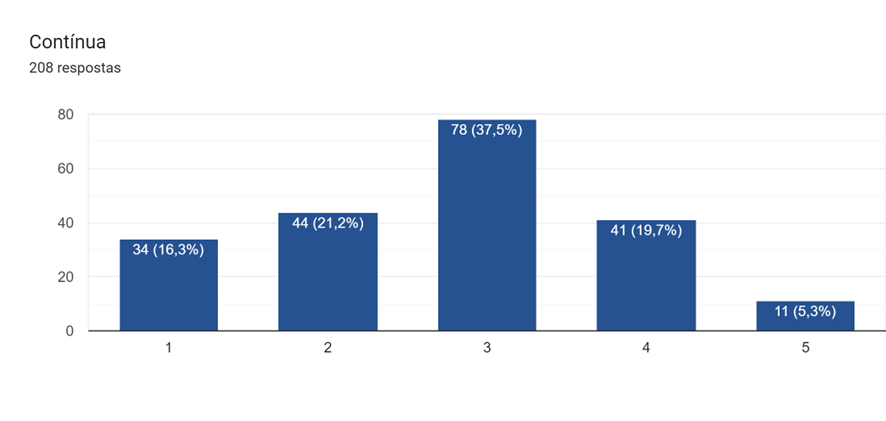
\includegraphics[width=\textwidth]{files/img/2.02!3-organizacao/2.02!3.1.4-forms/6.3-Opiniao-Continua}
  \end{MyCenteredFigure}

  \begin{MyCenteredFigure} \caption{Notas dadas para a característica: eficiente} \label{fig:6.4-Opiniao-Eficiente}
    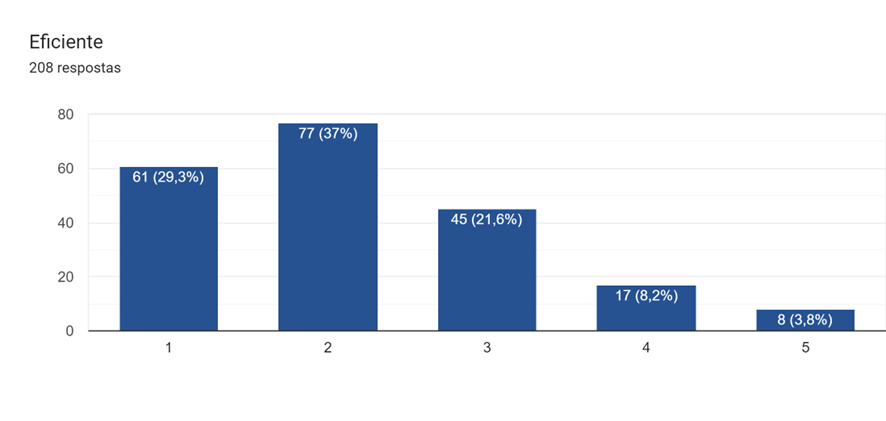
\includegraphics[width=\textwidth]{files/img/2.02!3-organizacao/2.02!3.1.4-forms/6.4-Opiniao-Eficiente}
  \end{MyCenteredFigure}

  \begin{MyCenteredFigure} \caption{Notas dadas para a característica: distribuída} \label{fig:6.5-Opiniao-Distribuida}
    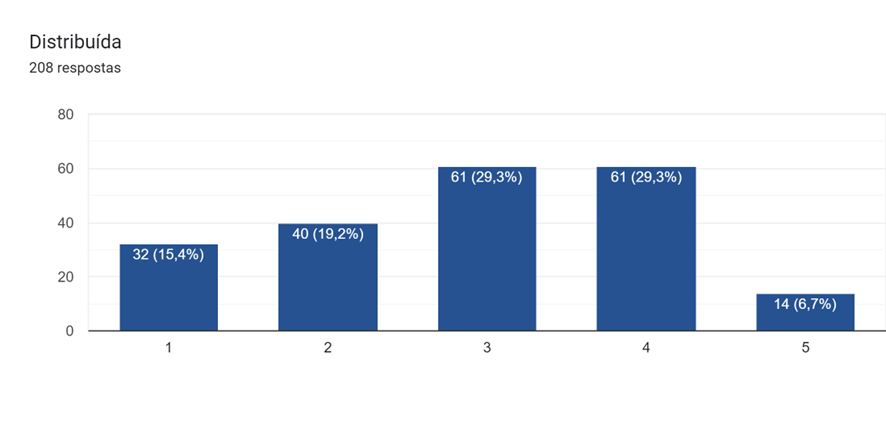
\includegraphics[width=\textwidth]{files/img/2.02!3-organizacao/2.02!3.1.4-forms/6.5-Opiniao-Distribuida}
  \end{MyCenteredFigure}

  \begin{MyCenteredFigure} \caption{Notas dadas para a característica: satisfatória} \label{fig:6.6-Opiniao-Satisfatoria}
    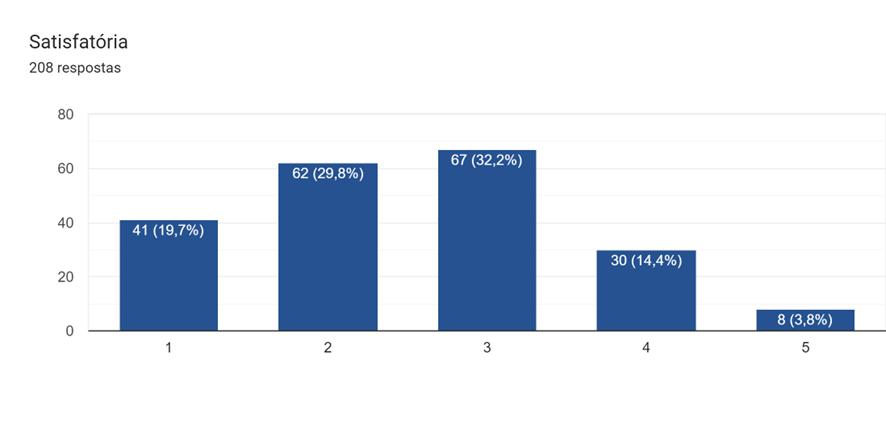
\includegraphics[width=\textwidth]{files/img/2.02!3-organizacao/2.02!3.1.4-forms/6.6-Opiniao-Satisfatoria}
  \end{MyCenteredFigure}
  \end{comment}

  De uma forma geral, conseguimos ver todos os gráficos com menos de 7\% dos respondentes dando nota 5 em cada uma das características, A maioria das respostas tende a estar entre 1 e 3, sendo exceção apenas no caso da característica ``distribuída'', que por sua vez apresenta uma elevada quantidade de notas 4, sendo referente a 29,3\% dos respondentes.

  Como forma tabular, temos, na \autoref{table:6.0-Opiniao}, as respostas dos alunos, seguidas das médias por característica.

  \begin{CenteredTable} \caption{Notas dadas às características da distribuição de disciplinas} \label{table:6.0-Opiniao}
    \begin{tabular}{| l | c c c c c | c |}
      \hline
      \multicolumn{1}{|c|}{\multirow{2}{*}{Opções}} &
      \multicolumn{5}{c|}{Notas}                    &
      \multicolumn{1}{|c|}{\multirow{2}{*}{Médias}}
      \\
      \multicolumn{1}{|c|}{}                        &
      \multicolumn{1}{c|}{1}                        &
      \multicolumn{1}{c|}{2}                        &
      \multicolumn{1}{c|}{3}                        &
      \multicolumn{1}{c|}{4}                        &
      \multicolumn{1}{c|}{5}                        &
      \multicolumn{1}{|c|}{}                                                       \\
      \hline
      Justa                                         & 59 & 69 & 52 & 17 & 10 & 2,3 \\
      Variada                                       & 40 & 65 & 64 & 26 & 12 & 2,5 \\
      Contínua                                      & 34 & 44 & 78 & 41 & 10 & 2,8 \\
      Eficiente                                     & 61 & 76 & 45 & 17 & 8  & 2,2 \\
      Distribuída                                   & 32 & 40 & 61 & 60 & 14 & 2,9 \\
      Satisfatória                                  & 40 & 61 & 68 & 30 & 8  & 2,5 \\
      \hline
    \end{tabular}
  \end{CenteredTable}

  Ao analisarmos a média de cada uma, podemos dizer que, em suma, há o visível desagrado do corpo discente quanto à distribuição de disciplinas semestrais, com ênfase nas duas piores notas que são 2,2 para ``eficiente'' e 2,3 para ``justa'' o que reforça a necessidade de aprimoramento do sistema atual.

  \section*{Respostas qualitativas} \label{sec:Respostas qualitativas}

  Por fim, havia um espaço livre no formulário para que os alunos pudessem expressar suas opiniões de forma mais livre. Após a leitura de todas e a filtragem das opiniões expressas, resumem-se em 4 parabenizações pelo desenvolvimento do presente projeto, 18 reclamações e 16 sugestões. Dentre elas, algumas apresentaram maior recorrência, sendo elas:

  \begin{itemize}
    \item 5 reclamações sobre a usual oferta de disciplinas separadas entre pares e ímpares;
    \item 4 reclamações sobre o Sistema Acadêmico, principalmente sobre não ser capaz de suportar a carga nos momentos iniciais de inscrição de disciplinas;
    \item 3 sugestões de ofertas de disciplinas recorrentemente, com ênfase nas disciplinas de matemática/que contemplam diversos cursos/com alta taxa de reprovação;
    \item 3 sugestões de mais oferta de disciplinas no período de verão;
    \item 2 sugestões de que inscrições em matérias do semestre atual esperado do aluno fossem feitas automaticamente, mas ainda permitindo a sua exclusão caso desejado;
    \item 1 sugestão de criação de um formulário de demanda no acadêmico que computasse a intenção de matrícula dos alunos.
  \end{itemize}

  Abaixo estão dispostas algumas das respostas obtidas:

  \begin{itemize}
    \item ``A estrutura curricular deveria ser predefinida, automatizando a matrícula dos alunos nas disciplinas correspondentes aos seus períodos acadêmicos. No entanto, permitir-se-ia a edição do cronograma por parte dos alunos, caso desejem quitar pendências de períodos anteriores ou disciplinas antecipadas. Além disso, disciplinas que abrangem múltiplos cursos devem ser oferecidas em ambos os semestres.

          Para melhorar a oferta de disciplinas, seria aconselhável ampliar a disponibilidade de disciplinas durante o período de verão. Isso facilitaria o acesso dos alunos ao estágio obrigatório durante as férias, viabilizando a conclusão dessa etapa essencial do curso. Reduzir o número de créditos necessários para antecipar a realização do estágio também se mostraria benéfico, visto que atualmente, a conclusão dessa matéria com apenas 9 créditos pendentes inviabiliza a possibilidade de antecipação antes do 9º período. Considera-se viável permitir essa antecipação a partir do 7º período.

          [...]
          Essas melhorias no sistema acadêmico [...] agilizariam a trajetória do estudante, permitindo maior flexibilidade na escolha e realização de disciplinas [...].''
    \item ``Existe muita desorganização em relação a grade, disciplinas e sistema acadêmico por parte dos coordenadores dos cursos. Me inscrevi numa matéria que tinha requisito de acordo com o plano pedagógico, mas tanto na grade como no sistema acadêmico não tinha pré-requisito nenhum. Tive que desistir da matéria pela dificuldade, até porque a matéria que era pré-requisito eu perdi. Detalhe: Outras pessoas perderam na matéria pré-requisito e continuaram fazendo a matéria desse período.''
    \item ``Acho que as coordenações precisam estabelecer um melhor diálogo com os alunos. Esse sistema de período par e Ímpar na UENF é antigo e perpetua um comodismo dos professores que acabam não ofertando disciplinas todos os semestres e prejudicando os alunos nas escolhas de matérias optativas, eletivas, instrumentais e obrigatórias tendo que esperar um ano para realizar a disciplina caso você não consiga fazer por choque de horário e/ou reprovação.''
  \end{itemize}

  \section*{Conclusões} \label{sec:Conclusões}

  Por fim, entendemos que, além das insatisfações dormentes por parte dos gestores e criadores de grades horárias, os alunos também se mostram insatisfeitos com a atual estrutura de distribuição de disciplinas semestrais. Os interesses dos alunos se mostram em sua maioria alinhados com os interesses dos gestores, onde ambos visam reduzir a quantidade de atrasos na progressão do curso.

  \chapter{Código-Fonte da Monografia} \label{apendice:CodigoFonte}

  Como forma mais prática é sugerida de acesso ao código-fonte da monografia, recomenda-se acessar o \LinkToURL{\LinkCodigoFonteSistema}{repositório do GitHub}, nele constará o código-fonte mais atualizado do sistema. Caso por algum motivo o link não esteja funcionando apropriadamente, está disponibilizado também na guia de Anexos do documento PDF deste trabalho o código-fonte do sistema. Para acessá-lo, basta procurar a aba de anexos em algum leitor de PDF que suporte anexos, como por exemplo o \LinkToURL{\LinkAdobeReader}{Adobe Reader}, ou clique \textattachfile{files/codigos/CodigoFonteSistema.rar}{aqui}. Como em alguns casos o leitor de PDF pode não ter suporte para abrir arquivos compactados, \textattachfile{files/codigos/CodigoFonteSistema.rar.RemovaEstaPartaParaAcessarOCodigo}{essa} é outra alternativa.

  Além do código do sistema, também está disponível o código-fonte \LaTeX deste documento, também num \LinkToURL{\LinkCodigoFonteMonografia}{repositório do GitHub}, porém nesse caso, talvez seja necessário passar por uma burocracia antes, visto que o primeiro link é de um repositório contido em uma organização privada, sendo necessário primeiro obter acesso a ela através de um procedimento descrito \LinkToURL{\LinkDisciplinas}{aqui}. Caso prefira, assim como no caso anterior, disponho também o código-fonte \LaTeX deste documento na guia de Anexos do documento PDF \textattachfile{files/codigos/CodigoFonteLaTeX.rar}{aqui}, ou \textattachfile{files/codigos/CodigoFonteLaTeX.rar}{aqui}.

  \chapter{Formulário de pesquisa editável} \label{apendice:FormularioPesquisaQuantitativaEditavel}

  Abaixo está o formulário de pesquisa quantitativa de alunos da UENF sobre distribuição e oferta de disciplinas. Este formulário foi feito em \LaTeX{} e é editável, podendo ser preenchido e enviado por e-mail. Para preenchê-lo, basta clicar no campo desejado e preencher com as informações solicitadas. Para enviar o formulário, clique no botão ``Enviar''.

  \begin{Form}[action=mailto:joaovitorfd2000@gmail.com, encoding=html, method=post]

    Pesquisa quantitativa de alunos da UENF sobre distribuição e oferta de disciplinas

    \section*{Pesquisa quantitativa de alunos da UENF sobre distribuição e oferta de disciplinas}

    Olá! Desde já agradeço por ceder em torno de 4 minutos do seu tempo para responder a este formulário usando o seu e-mail institucional. Considerando que nosso tempo é valioso, vamos direto ao objetivo:

    Me chamo João Vítor Fernandes Dias, estudante de Ciência da Computação na UENF, e estou fazendo minha Monografia. Ela trata da elaboração de um sistema para a coordenação de curso poder analisar mais facilmente quais são as disciplinas que serão disponibilizadas a cada semestre e a quais salas e professores serão atribuídas.

    O objetivo da minha monografia é conseguir tornar mais eficiente a distribuição das disciplinas, para que se resulte em um conjunto de disciplinas ofertadas com melhor qualidade. Espera-se com isso que as demandas de disciplina dos alunos sejam melhor atendidas, assim como as preferências de horários dos professores.

    Este formulário tem como objetivo avaliar a sua satisfação em relação ao processo de inscrição semestral nas disciplinas.

    \section*{Sobre você}

    Nesta seção, peço que informe algumas características suas para que a análise estatística se torne mais rica.

    \begin{enumerate}
      \QuestionNameOptions{Qual o seu curso?}{curso}
      {
        1. Administração Pública,
        2. Agronomia,
        3. Biologia (Licenciatura),
        4. Ciência da Computação,
        5. Ciências Biológicas (bacharelado),
        6. Ciências Sociais,
        7. Engenharia Civil,
        8. Engenharia de Exploração e Produção de Petróleo,
        9. Engenharia de Produção,
        10. Engenharia Metalúrgica,
        11. Engenharia Meteorológica,
        12. Física (licenciatura),
        13. Matemática (Licenciatura),
        14. Medicina Veterinária,
        15. Pedagogia (Licenciatura),
        16. Química (Licenciatura),
        17. Zootecnia,
        18. Outro,
      }
      \QuestionNameOptions{Em que ano você ingressou na UENF?}{anoIngresso}
      { 2023, 2022, 2021, 2020, 2019, 2018, 2017, 2016, 2015, 2014, 2013, Outro }
    \end{enumerate}

    \section*{Pesquisa de satisfação}

    Agora serão feitas algumas perguntas em relação à sua satisfação com algumas características da Universidade.

    Abaixo, estão algumas perguntas gerais em relação à sua satisfação com a distribuição de disciplinas semestralmente.

    \begin{enumerate}
      \ChoiceMenuSNO{\textbf{Salas}: Você já teve que mudar de sala por falta de algum acessório como quadro, projetor ou monitor?}{SalasAcessorios}
      \ChoiceMenuSNO{\textbf{Salas}: Você já teve aula cuja sala não dispunha de carteiras o suficiente?}{SalasCarteiras}
      \ChoiceMenuSNO{\textbf{Vagas}: Você já quis entrar em uma disciplina, mas ela não tinha vaga?}{VagasDisciplinas}
      \ChoiceMenuSNO{\textbf{Vagas}: Você já ficou acordado após meia-noite por medo de não ter vaga para as disciplinas que deseja cursar?}{VagasNoite}
      \ChoiceMenuSNO{\textbf{Conflitos}: Você já deixou de se inscrever em uma disciplina por causa de conflito de horário?}{Conflitos}
      \ChoiceMenuSNO{\textbf{Preferências}: Você já preferiu não se inscrever em uma disciplina para cursá-la em outro momento mais oportuno?}{Preferências}
      \ChoiceMenuSNO{\textbf{Opiniões}: Você acha que a universidade deveria oferecer horários diferentes para as disciplinas mais demandadas para evitar conflitos com outras disciplinas?}{Opiniões}
    \end{enumerate}

    \section*{Preferências pessoais}

    Esta seção visa saber um pouco mais sobre as suas preferências pessoais quanto a escolha das disciplinas ofertadas.

    \begin{enumerate}
      \item Você prefere disciplinas distribuídas ao longo da semana ou acumuladas em poucos dias?
            \FormInNewLine{
              \ChoiceMenu[print, combo, name=distribuiçãoDisciplinasNaSemana]{ }
              {
                1. Distribuídas ao longo da semana,
                2. Preferencialmente ao longo da semana,
                3. Não tenho preferência,
                4. Preferencialmente acumulada em poucos dias,
                5. Acumuladas em poucos dias,
              }
            }

      \item Você prefere disciplinas na parte da manhã ou na parte da tarde?
            \FormInNewLine{
              \ChoiceMenu[print, combo, name=distribuiçãoDisciplinasNoDia]{ }
              {
                1. Na parte da manhã,
                2. Preferencialmente na parte da manhã,
                3. Não tenho preferência,
                4. Preferencialmente na parte da tarde,
                5. Na parte da tarde,
              }

            }
      \item Como você lida com conflitos de horário entre as disciplinas que deseja cursar?
            \begin{itemize}
              \MyCheckbox{Escolho a mais difícil}{dificil}
              \MyCheckbox{Escolho a mais fácil}{facil}
              \MyCheckbox{Escolho a que tem mais créditos}{creditos}
              \MyCheckbox{Escolho a que prefiro}{prefiro}
              \MyCheckbox{Escolho a que ``prende'' mais matérias}{prende}
              \MyCheckbox{Escolho a disciplina mais concorrida}{concorrida}
              \item \TextField[name=ComentarioConflito, width=0.8\linewidth]{Outro...}
            \end{itemize}
    \end{enumerate}

    \section*{Experiências passadas com atrasos e disciplinas}

    Aqui estão algumas perguntas relacionadas à divergência entre o período esperado de conclusão das disciplinas VS o período em que elas de fato são realizadas.

    \begin{enumerate}
      \ChoiceMenuPeriodos{Quanto tempo (em períodos) você já teve que esperar para fazer uma disciplina da sua grade?}{TempoEspera}
      \ChoiceMenuPeriodos{Qual foi a quantidade máxima de períodos que você se distanciou de uma disciplina de determinado período?}{DistanciaPeriodos}
    \end{enumerate}

    \section*{Você acha que a distribuição de disciplinas semestrais é...}

    \begin{enumerate}
      \ChoiceMenuDdNcC{Justa (feita de acordo a atender os desejos da maioria)}{Justa}
      \ChoiceMenuDdNcC{Variada (bem diversa e abrange diversos interesses)}{Variada}
      \ChoiceMenuDdNcC{Contínua (oferecida de forma a ter aulas sequenciais)}{Contínua}
      \ChoiceMenuDdNcC{Eficiente (bem sucedida em atender aos desejos dos alunos)}{Eficiente}
      \ChoiceMenuDdNcC{Distribuída (bem espaçada ao longo da semana)}{Distribuída}
      \ChoiceMenuDdNcC{Satisfatória (agradável aos meus desejos pessoais)}{Satisfatória}
    \end{enumerate}

    \section*{Opcional}

    Por fim, deixo aqui um espaço caso deseje compartilhar algum comentário, opinião ou sugestão quanto ao meu trabalho ou formulário.

    Escreva aqui caso haja algo que gostaria de comentar, opinar ou sugerir. Tudo bem deixar em branco, suas informações já foram de grande ajuda.

    \TextField[multiline=true, width=0.8\linewidth, name=comentario]{ }

    \Reset{Resetar}
    \Submit{Enviar}

  \end{Form}

  \chapter{Formulário de pesquisa textual} \label{apendice:FormularioPesquisaQuantitativaTextual}

  Pesquisa quantitativa de alunos da UENF sobre distribuição e oferta de disciplinas

  \section*{Pesquisa quantitativa de alunos da UENF sobre distribuição e oferta de disciplinas}

  Olá! Desde já agradeço por ceder em torno de 4 minutos do seu tempo para responder a este formulário usando o seu e-mail institucional. Considerando que nosso tempo é valioso, vamos direto ao objetivo:

  Me chamo João Vítor Fernandes Dias, estudante de Ciência da Computação na UENF, e estou fazendo minha Monografia. Ela trata da elaboração de um sistema para a coordenação de curso poder analisar mais facilmente quais são as disciplinas que serão disponibilizadas a cada semestre e a quais salas e professores serão atribuídas.

  O objetivo da minha monografia é conseguir tornar mais eficiente a distribuição das disciplinas, para que se resulte em um conjunto de disciplinas ofertadas com melhor qualidade. Espera-se com isso que as demandas de disciplina dos alunos sejam melhor atendidas, assim como as preferências de horários dos professores.

  Este formulário tem como objetivo avaliar a sua satisfação em relação ao processo de inscrição semestral nas disciplinas.

  \section*{Sobre você}

  Nesta seção, peço que informe algumas características suas para que a análise estatística se torne mais rica.

  \begin{itemize}
    \item \textbf{Pergunta:} Qual o seu curso?
    \item \textbf{Opções de resposta}
          \begin{enumerate}
            \item Administração Pública
            \item Agronomia
            \item Biologia (Licenciatura)
            \item Ciência da Computação
            \item Ciências Biológicas (bacharelado)
            \item Ciências Sociais
            \item Engenharia Civil
            \item Engenharia de Exploração e Produção de Petróleo
            \item Engenharia de Produção
            \item Engenharia Metalúrgica
            \item Engenharia Meteorológica
            \item Física (licenciatura)
            \item Matemática (Licenciatura)
            \item Medicina Veterinária
            \item Pedagogia (Licenciatura)
            \item Química (Licenciatura)
            \item Zootecnia
            \item Outro
          \end{enumerate}
  \end{itemize}

  \begin{itemize}
    \item \textbf{Pergunta:} Em que ano você ingressou na UENF?
    \item \textbf{Opções de resposta}
          \begin{enumerate}
            \item 2023
            \item 2022
            \item 2021
            \item 2020
            \item 2019
            \item 2018
            \item 2017
            \item 2016
            \item 2015
            \item 2014
            \item 2013
            \item Outro
          \end{enumerate}
  \end{itemize}

  \section*{Pesquisa de satisfação}

  Agora serão feitas algumas perguntas em relação à sua satisfação com algumas características da Universidade.

  Abaixo, estão algumas perguntas gerais em relação à sua satisfação com a distribuição de disciplinas semestralmente.

  \begin{itemize}
    \item \textbf{Perguntas}
          \begin{enumerate}
            \item Salas: Você já teve que mudar de sala por falta de algum acessório como quadro, projetor ou monitor?
            \item Salas: Você já teve aula cuja sala não dispunha de carteiras o suficiente?
            \item Vagas: Você já quis entrar em uma disciplina, mas ela não tinha vaga?
            \item Vagas: Você já ficou acordado após meia-noite por medo de não ter vaga para as disciplinas que deseja cursar?
            \item Conflitos: Você já deixou de se inscrever em uma disciplina por causa de conflito de horário?
            \item Preferências: Você já preferiu não se inscrever em uma disciplina para cursá-la em outro momento mais oportuno?
            \item Opiniões: Você acha que a universidade deveria oferecer horários diferentes para as disciplinas mais demandadas para evitar conflitos com outras disciplinas?
          \end{enumerate}
    \item \textbf{Opções de resposta}
          \begin{enumerate}
            \item Sim
            \item Não
            \item Outro
          \end{enumerate}
  \end{itemize}

  \section*{Preferências pessoais}

  Esta seção visa saber um pouco mais sobre as suas preferências pessoais quanto a escolha das disciplinas ofertadas.

  \begin{itemize}
    \item \textbf{Pergunta:} Você prefere disciplinas distribuídas ao longo da semana ou acumuladas em poucos dias?
    \item \textbf{Opções de resposta}
          \begin{enumerate}
            \item Distribuídas ao longo da semana
            \item $\sim$
            \item Não tenho preferência
            \item $\sim$
            \item Acumuladas em poucos dias
          \end{enumerate}
  \end{itemize}

  \begin{itemize}
    \item \textbf{Pergunta:} Você prefere disciplinas na parte da manhã ou na parte da tarde?
    \item \textbf{Opções de resposta}
          \begin{enumerate}
            \item na parte da manhã
            \item $\sim$
            \item Não tenho preferência
            \item $\sim$
            \item na parte da tarde
          \end{enumerate}
  \end{itemize}

  \begin{itemize}
    \item Como você lida com conflitos de horário entre as disciplinas que deseja cursar?
    \item \textbf{Opções de resposta} (Permite múltiplas escolhas)
          \begin{itemize}
            \item Escolho a mais difícil
            \item Escolho a mais fácil
            \item Escolho a que tem mais créditos
            \item Escolho a que prefiro
            \item Escolho a que ``prende'' mais matérias
            \item Escolho a disciplina mais concorrida
            \item Outro...
          \end{itemize}
  \end{itemize}

  \section*{Experiências passadas com atrasos e disciplinas}

  Aqui estão algumas perguntas relacionadas à divergência entre o período esperado de conclusão das disciplinas VS o período em que elas de fato são realizadas.

  \begin{itemize}
    \item \textbf{Pergunta:} Quanto tempo (em períodos) você já teve que esperar para fazer uma disciplina da sua grade?
    \item Descrição: Exemplo hipotético: estou no 6º período e estou desde o 4º período tentando me inscrever em uma disciplina, mas ela não foi oferecida ou não teve vaga, então tive que esperar 2 períodos.
    \item \textbf{Opções de resposta}: 0, 1, 2, 3, 4, 5, 6, 7, 8, 9, 10
  \end{itemize}

  \begin{itemize}
    \item \textbf{Pergunta:} Qual foi a quantidade máxima de períodos que você se distanciou de uma disciplina de determinado período?
    \item Descrição: Exemplo hipotético: estou no 6º período da faculdade, mas ainda estou cursando uma disciplina do 3º período, pois escolhi não fazer antes, ou ainda não obtive a aprovação, logo, me distanciei 3 períodos do esperado.
    \item \textbf{Opções de resposta}: 0, 1, 2, 3, 4, 5, 6, 7, 8, 9, 10
  \end{itemize}

  \section*{Você acha que a distribuição de disciplinas semestrais é...}

  \begin{itemize}
    \item Classificações
          \begin{itemize}
            \item Justa (feita de acordo a atender os desejos da maioria)
            \item Variada (bem diversa e abrange diversos interesses)
            \item Contínua (oferecida de forma a ter aulas sequenciais)
            \item Eficiente (bem sucedida em atender aos desejos dos alunos)
            \item Distribuída (bem espaçada ao longo da semana)
            \item Satisfatória (agradável aos meus desejos pessoais)
          \end{itemize}
    \item \textbf{Descrição:} Exemplo hipotético: estou no 6º período da faculdade, mas ainda estou cursando uma disciplina do 3º período, pois escolhi não fazer antes, ou ainda não obtive a aprovação, logo, me distanciei 3 períodos do esperado.
          \begin{enumerate}
            \item Discordo completamente
            \item $\sim$
            \item $\sim$
            \item $\sim$
            \item Concordo completamente
          \end{enumerate}
  \end{itemize}

  \section*{Opcional}

  Por fim, deixo aqui um espaço caso deseje compartilhar algum comentário, opinião ou sugestão quanto ao meu trabalho ou formulário.

  Escreva aqui caso haja algo que gostaria de comentar, opinar ou sugerir. Tudo bem deixar em branco, suas informações já foram de grande ajuda.

  \begin{itemize}
    \item Campo de texto livre
  \end{itemize}

  \chapter{Exemplo de \textit{template.yaml}} \label{apendice:ExemploTemplateYAML}

  O arquivo \textit{template.yaml} é um arquivo de configuração do \textit{AWS SAM} que define como a aplicação será construída e como será feito o deploy dela. Abaixo está um exemplo deste arquivo.

  \lstinputlisting[language={YAML}, captionpos={t}, label={code:template}, caption={Exemplo de \textit{template.yaml}}]{files/codigos/AWS_SAM.yaml}

\end{apendicesenv}
